%!TEX program = xelatex
\documentclass[11pt,article,oneside]{memoir}
\usepackage{org-preamble-xelatex}
\DisemulatePackage{setspace}
\usepackage{setspace}
% \input{vc}

\usepackage{longtable}

\usepackage{graphicx}
% We will generate all images so they have a width \maxwidth. This means
% that they will get their normal width if they fit onto the page, but
% are scaled down if they would overflow the margins.
\makeatletter
\def\maxwidth{\ifdim\Gin@nat@width>\linewidth\linewidth
\else\Gin@nat@width\fi}
\makeatother
\let\Oldincludegraphics\includegraphics
\renewcommand{\includegraphics}[1]{\Oldincludegraphics[width=\maxwidth]{#1}}

\title{\bigskip \bigskip How Does the State Speak about Globalisation? A Quantitative Text-Mining
Approach}

%\author{}

\author{\Large Justin Murphy\vspace{0.05in} \newline\normalsize\emph{University of Southampton} \newline\footnotesize \url{j.murphy@soton.ac.uk}\vspace*{0.2in}\newline }

%\author{Justin Murphy (University of Southampton)}

\date{}


\begin{document}  
\setkeys{Gin}{width=1\textwidth} 	
\setromanfont[Mapping=tex-text,Numbers=OldStyle]{Georgia} 
\setsansfont[Mapping=tex-text]{Gill Sans} 
\setmonofont[Mapping=tex-text,Scale=0.8]{Consolas}
\chapterstyle{article-2}

\doublespacing


\maketitle



\begin{abstract}

\noindent Scholars argue that the concept of ``globalisation'' is strategically
deployed by governments to rationalise their actions (Hay and Rosamond
2011). This article is the first large-scale quantitative assessment of
this argument, using text-mining and machine learning techniques to
analyze more than 60,000 government web pages. Specifically, this
article exploits the newly released United Kingdom Government Web
Archive to analyze a random sample of web pages published across the
entire UK government web system between 2000 and 2013.

\end{abstract}


I requested 150,000 web pages, received 67k and about 1k were errors.
Thus, the final sample consists of a corpus of dtm

\pagebreak

\subsubsection{Descriptive Statistics}\label{descriptive-statistics}

\begin{figure}[htbp]
\centering
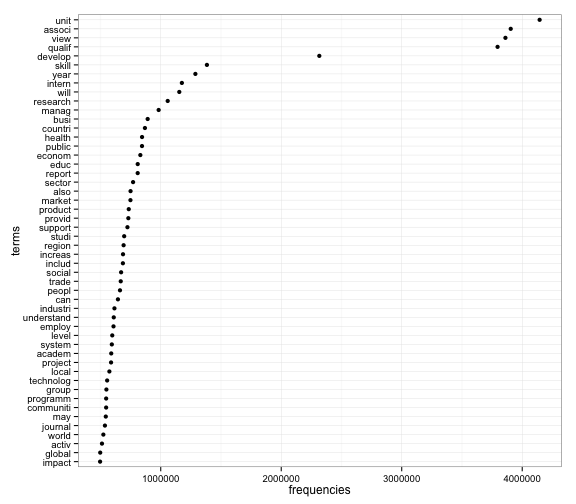
\includegraphics{figure/globalisation_frequency_plot.png}
\caption{Most frequent terms}
\end{figure}

\pagebreak

\paragraph{Correlated terms}\label{correlated-terms}

\begin{longtable}[c]{@{}cc@{}}
\toprule\addlinespace
\begin{minipage}[b]{0.14\columnwidth}\centering
Terms
\end{minipage} & \begin{minipage}[b]{0.17\columnwidth}\centering
Correlation
\end{minipage}
\\\addlinespace
\midrule\endhead
\begin{minipage}[t]{0.14\columnwidth}\centering
world
\end{minipage} & \begin{minipage}[t]{0.17\columnwidth}\centering
0.78
\end{minipage}
\\\addlinespace
\begin{minipage}[t]{0.14\columnwidth}\centering
countri
\end{minipage} & \begin{minipage}[t]{0.17\columnwidth}\centering
0.66
\end{minipage}
\\\addlinespace
\begin{minipage}[t]{0.14\columnwidth}\centering
economi
\end{minipage} & \begin{minipage}[t]{0.17\columnwidth}\centering
0.63
\end{minipage}
\\\addlinespace
\begin{minipage}[t]{0.14\columnwidth}\centering
threat
\end{minipage} & \begin{minipage}[t]{0.17\columnwidth}\centering
0.62
\end{minipage}
\\\addlinespace
\begin{minipage}[t]{0.14\columnwidth}\centering
increas
\end{minipage} & \begin{minipage}[t]{0.17\columnwidth}\centering
0.61
\end{minipage}
\\\addlinespace
\begin{minipage}[t]{0.14\columnwidth}\centering
goal
\end{minipage} & \begin{minipage}[t]{0.17\columnwidth}\centering
0.6
\end{minipage}
\\\addlinespace
\begin{minipage}[t]{0.14\columnwidth}\centering
key
\end{minipage} & \begin{minipage}[t]{0.17\columnwidth}\centering
0.6
\end{minipage}
\\\addlinespace
\begin{minipage}[t]{0.14\columnwidth}\centering
agricultur
\end{minipage} & \begin{minipage}[t]{0.17\columnwidth}\centering
0.59
\end{minipage}
\\\addlinespace
\begin{minipage}[t]{0.14\columnwidth}\centering
also
\end{minipage} & \begin{minipage}[t]{0.17\columnwidth}\centering
0.59
\end{minipage}
\\\addlinespace
\begin{minipage}[t]{0.14\columnwidth}\centering
develop
\end{minipage} & \begin{minipage}[t]{0.17\columnwidth}\centering
0.58
\end{minipage}
\\\addlinespace
\begin{minipage}[t]{0.14\columnwidth}\centering
particular
\end{minipage} & \begin{minipage}[t]{0.17\columnwidth}\centering
0.57
\end{minipage}
\\\addlinespace
\begin{minipage}[t]{0.14\columnwidth}\centering
econom
\end{minipage} & \begin{minipage}[t]{0.17\columnwidth}\centering
0.55
\end{minipage}
\\\addlinespace
\begin{minipage}[t]{0.14\columnwidth}\centering
mani
\end{minipage} & \begin{minipage}[t]{0.17\columnwidth}\centering
0.55
\end{minipage}
\\\addlinespace
\begin{minipage}[t]{0.14\columnwidth}\centering
privat
\end{minipage} & \begin{minipage}[t]{0.17\columnwidth}\centering
0.55
\end{minipage}
\\\addlinespace
\begin{minipage}[t]{0.14\columnwidth}\centering
coher
\end{minipage} & \begin{minipage}[t]{0.17\columnwidth}\centering
0.54
\end{minipage}
\\\addlinespace
\begin{minipage}[t]{0.14\columnwidth}\centering
competit
\end{minipage} & \begin{minipage}[t]{0.17\columnwidth}\centering
0.54
\end{minipage}
\\\addlinespace
\begin{minipage}[t]{0.14\columnwidth}\centering
primari
\end{minipage} & \begin{minipage}[t]{0.17\columnwidth}\centering
0.53
\end{minipage}
\\\addlinespace
\begin{minipage}[t]{0.14\columnwidth}\centering
educ
\end{minipage} & \begin{minipage}[t]{0.17\columnwidth}\centering
0.52
\end{minipage}
\\\addlinespace
\begin{minipage}[t]{0.14\columnwidth}\centering
exampl
\end{minipage} & \begin{minipage}[t]{0.17\columnwidth}\centering
0.52
\end{minipage}
\\\addlinespace
\begin{minipage}[t]{0.14\columnwidth}\centering
howev
\end{minipage} & \begin{minipage}[t]{0.17\columnwidth}\centering
0.52
\end{minipage}
\\\addlinespace
\begin{minipage}[t]{0.14\columnwidth}\centering
integr
\end{minipage} & \begin{minipage}[t]{0.17\columnwidth}\centering
0.52
\end{minipage}
\\\addlinespace
\begin{minipage}[t]{0.14\columnwidth}\centering
success
\end{minipage} & \begin{minipage}[t]{0.17\columnwidth}\centering
0.52
\end{minipage}
\\\addlinespace
\begin{minipage}[t]{0.14\columnwidth}\centering
capac
\end{minipage} & \begin{minipage}[t]{0.17\columnwidth}\centering
0.5
\end{minipage}
\\\addlinespace
\begin{minipage}[t]{0.14\columnwidth}\centering
dfid
\end{minipage} & \begin{minipage}[t]{0.17\columnwidth}\centering
0.5
\end{minipage}
\\\addlinespace
\begin{minipage}[t]{0.14\columnwidth}\centering
millennium
\end{minipage} & \begin{minipage}[t]{0.17\columnwidth}\centering
0.5
\end{minipage}
\\\addlinespace
\bottomrule
\end{longtable}

\pagebreak

\section{Appendix}\label{appendix}

\subsection{Diagnostics}\label{diagnostics}

\begin{figure}[htbp]
\centering
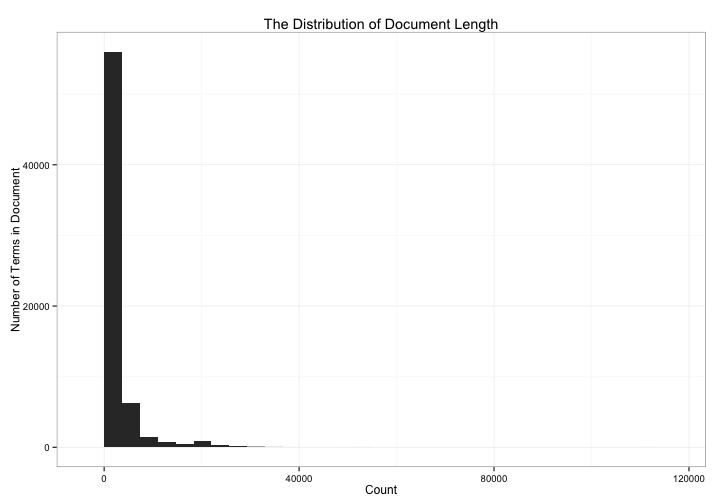
\includegraphics{figure/Document-Lengths.png}
\caption{Document lengths}
\end{figure}

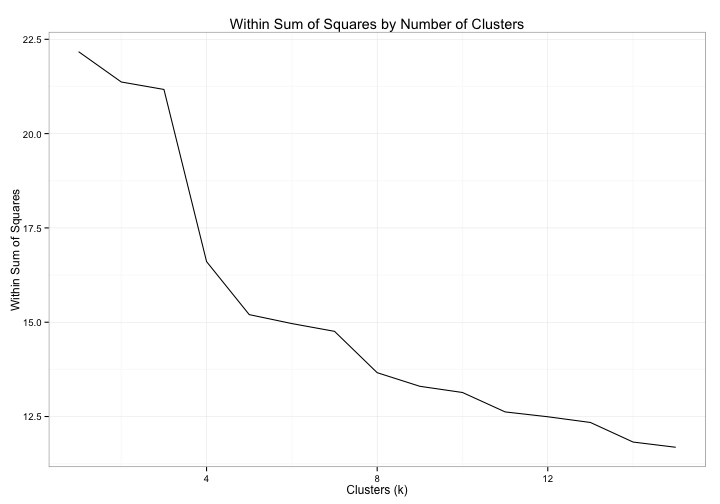
\includegraphics{figure/Cluster-Diagnostics1.png}
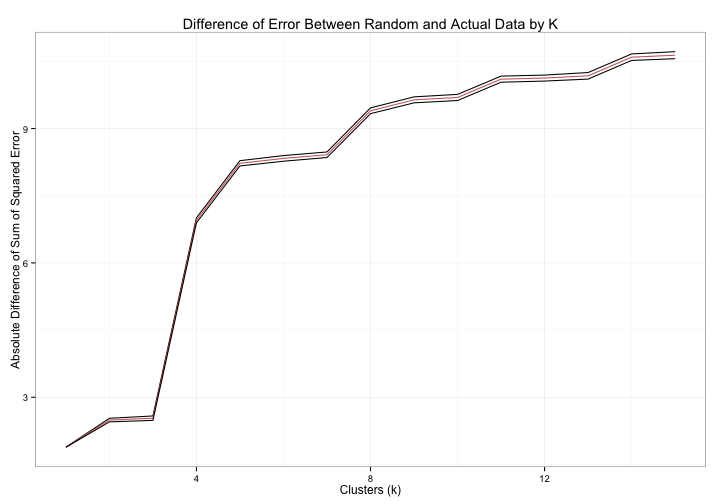
\includegraphics{figure/Cluster-Diagnostics2.png}

\pagebreak

\section{References}\label{references}

\setlength{\parindent}{-0.2in} \setlength{\leftskip}{0.2in}
\setlength{\parskip}{8pt} \vspace*{-0.2in} \noindent

Hay, Colin, and Ben Rosamond. 2011. ``Globalization, European
Integration and the Discursive Construction of Economic Imperatives.''
\emph{dx.doi.org.libproxy.temple.edu} 9(2): 147--67.
\url{http://www.tandfonline.com/doi/abs/10.1080/13501760110120192}.


\end{document}